\section{Metodología}
Se entiende por Inteligencia Artificial a una simulación de procesos computacionales cognitivos para que simulen el comportamiento de una mente humana, estos comportamientos abarcan diferentes áreas de investigación, como el aprendizaje, comunicación, percepción, razonamiento y la capacidad de desarrollarse en entornos más complejos.

\subsection{Red neuronal}
Una red neuronal es una herramienta derivada de la inteligencia artificial que utiliza modelos matemáticos para ser utilizada como un mecanismo de predicción del texto. Son una forma de hacer que las computadoras aprendan, donde la computadora aprende a realizar alguna tarea analizando ejemplos de entrenamiento. Por lo general, estos ejemplos han sido etiquetados previamente.\\\\
Las redes neuronales son modeladas vagamente asemejando el cerebro humano, esta consiste en miles de millones de nodos que realizan el procesamiento de la información los cuales están densamente interconectados.\\\\
La complejidad de las neuronas reales se abstrae mucho cuando se realiza el modelado de neuronas artificiales. Estas consisten básicamente en entradas, que se multiplican por pesos (fuerza de las respectivas señales), y luego calculada por una función matemática que determina la activación de la neurona. Otra función (que puede ser la de identidad) calcula la salida de la neurona artificial (a veces en dependencia de un cierto umbral). Las redes neuronales combinan neuronas artificiales para procesar información.\cite{neuronart}

\begin{figure}[h]
	\centering
	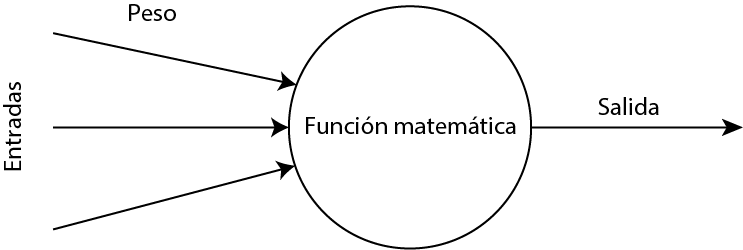
\includegraphics[width=8cm]{figuras/NeuronaArt.png}
	\caption{Neurona artificial.}
	\label{fig:Neurona artificial}
\end{figure}

\subsection{Recurrent Neural Network (RNN) – Long Short Term Memory (LSTM)}
Una red neuronal recurrente es un tipo de red neuronal artificial donde la salida de alguna capa en particular es salvada y sirve para retroalimentar la entrada de esta capa, lo cual ayuda a predecir futuras salidas de esta.
\begin{figure}[h]
	\centering
	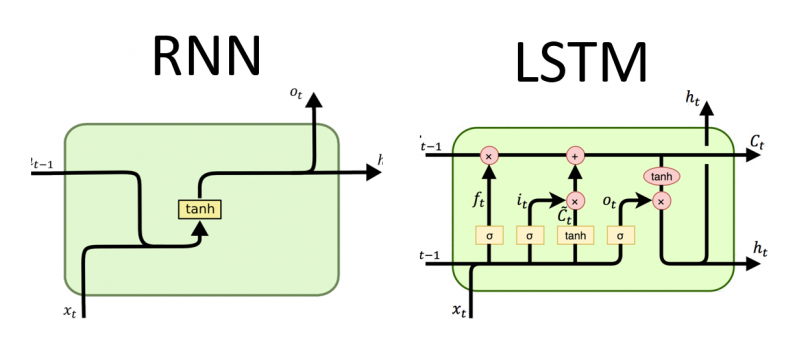
\includegraphics[width=8cm]{figuras/RnnLstm.png}
	\caption{Diagrama de las redes neuronales RNN y LSTM.}
	\label{fig:Diagrama de las redes neuronales RNN y LSTM}
\end{figure}
La primera capa está formada de la misma manera que la Feed-forward Neural Network, es decir, solo pasa la información que entra a la siguiente capa inmediata, posteriormente la siguiente capa con el paso del tiempo comenzará a retroalimentarse, pero manteniendo la propagación frontal. Haciendo uso de esta retroalimentación la capa en futuras operaciones puede realizar predicciones, si estas predicciones no son los resultados esperados, el sistema aprende y trabaja para corregir sus futuras predicciones.\cite{redneurnn}\\\\
Este tipo de redes neuronales se distinguen por su “memoria”, ya que toman información de entradas anteriores para influir en la entrada y salida actuales.

\subsection{Generación del modelo}

\subsubsection{Obtención del conjunto de datos}
El primer paso para poder empezar a trabajar con nuestro modelo fue obtener un conjunto de datos que cumpliera con las características que se necesitaban, por eso nos dimos a la tarea de buscar uno. En Kaggle \cite{kaggle1} se encontró un dataset llamado “Song lyrics for 6 musical genres” \cite{kaggleDataset} el cual contenía los datos necesarios y contaba con un total de 160,790 letras, las cuales pertenecían a 6 tipos de géneros musicales:
\begin{itemize}
	\item Rock
	\item Pop
	\item Hip Hop
	\item Samba
	\item Sertanejo
	\item Funk Carioca
\end{itemize}
Debido a que estas letras de canciones pertenecían a distintos géneros e idiomas se procedió a realizar una limpieza a la base de datos para quedarnos únicamente con las letras de canciones pertenecientes al genero pop y que estuvieran en el idioma inglés, además haciendo uso de la librería de “Pandas” y siguiendo el estándar de limpieza de datos: \cite{data_cleaning}
\begin{enumerate}
	\item Remover caracteres innecesarios
	\item Eliminar Duplicados
	\item Evitar errores ortográficos de similitud
	\item Convertir los tipos de dato
	\item Tratar los valores nulos o faltantes
\end{enumerate}
Se obtuvo como resultado un conjunto de datos útil, el cual solo cuenta con los datos necesarios para después poder tratarlos y utilizarlos para empezar el entrenamiento del modelo de la red neuronal, cabe destacar que este proceso es necesario hacerlo solo una vez para cada género musical ingresado, en caso de que se lleguen a necesitar más datos, será necesario repetir el proceso.
\subsubsection{Modelo}

\subsubsection{Entrenamiento}